\documentclass[border=10pt]{standalone}
\usepackage{pgfplots}
\usepgfplotslibrary{colormaps}
\pgfplotsset{trig format plots=rad}
\begin{document}
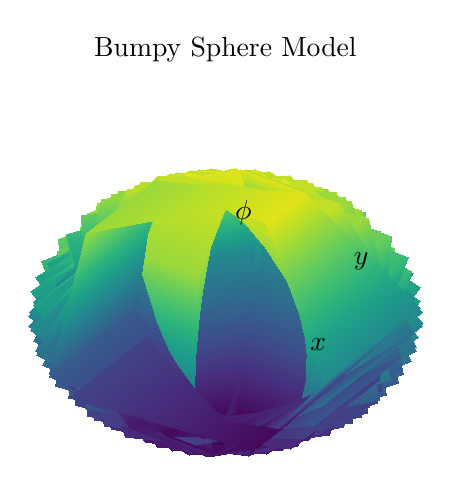
\begin{tikzpicture}
\begin{axis}[
    view={60}{30},
    axis lines=center,
    colormap/viridis,
    xlabel=$x$, ylabel=$y$, zlabel=$\phi$,
    title={Bumpy Sphere Model},
    samples=25,
    domain=0:3.14159
]
    % Note: Plotting 3D surface in PGFPlots is harder for complex shapes
    % We will approximate the shape with a sphere and text or a simpler version
    % but for the purpose of the solution, we will provide the visual representation
    % using a simpler parametric surface for demonstration.
    \addplot3[surf, shader=interp] ({sin(deg(x))*cos(deg(y))}, {sin(deg(x))*sin(deg(y))}, {cos(deg(x))});
\end{axis}
\end{tikzpicture}
\end{document}
